\begin{frame}
\frametitle{Définitions Fondamentales des Graphes}

\begin{tcolorbox}[colback=orange!10,colframe=orange!100!black,
    title=Un Graphe Non Connexe]
    Un \textbf{Graphe Non Connexe} contient des sommets isolés.
\end{tcolorbox}

\begin{figure}[H]
    \centering
    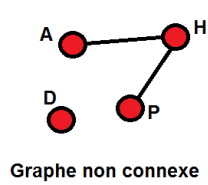
\includegraphics[width=0.5 \textwidth]{Figures/Graphe Non Connexe.PNG}
    \caption{Graphe Non Connexe}
    \label{fig:Graphe Non Connexe}
\end{figure}

\end{frame}


